% Compact PGFPlots panel for sampled surface15 BSC GEXIT derivative.
% Requires \usepackage{pgfplots} and \pgfplotsset{compat=1.18}.
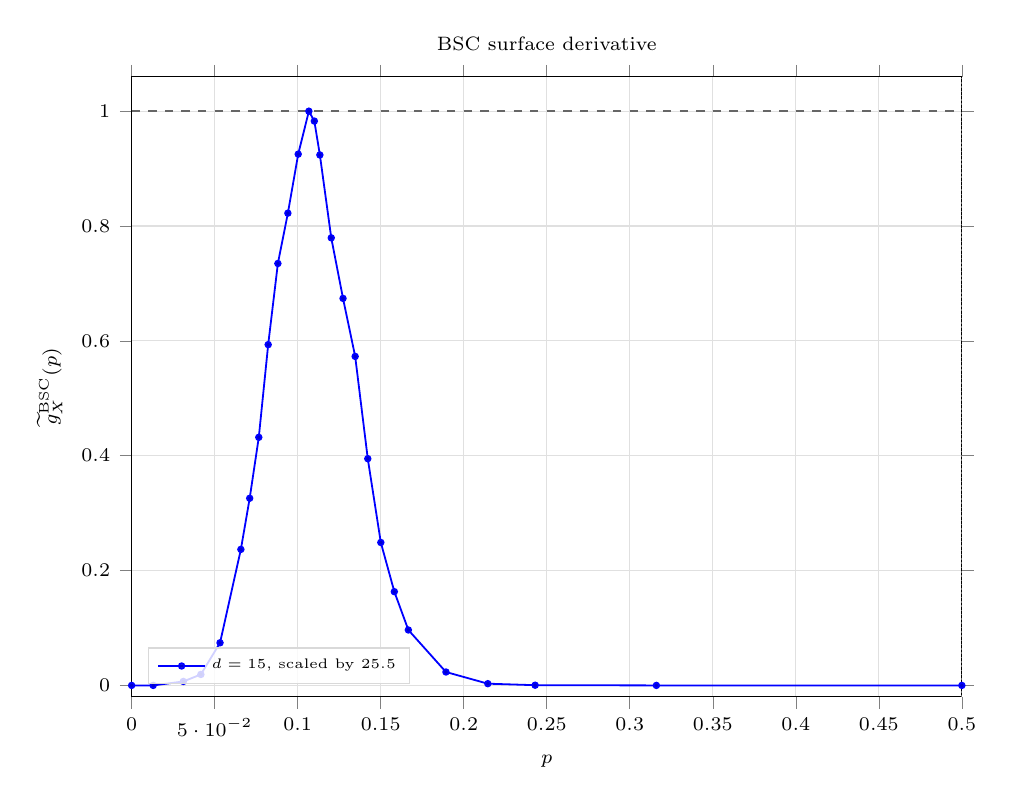
\begin{tikzpicture}
\begin{axis}[
  name=scaledBSCGEXITSurface15Axis,
  width=\linewidth,
  height=0.78\linewidth,
  title={BSC surface derivative},
  title style={font=\scriptsize},
  xlabel={$p$},
  ylabel={$\widetilde g_X^{\rm BSC}(p)$},
  xmin=0, xmax=0.5,
  ymin=-0.02, ymax=1.06,
  grid=both,
  major grid style={black!12},
  minor grid style={black!6},
  tick align=outside,
  tick label style={font=\scriptsize},
  label style={font=\scriptsize},
  legend cell align={left},
  legend style={draw=black!15, fill=white, fill opacity=0.82, text opacity=1, at={(0.02,0.02)}, anchor=south west, font=\tiny},
]
\addplot[black!60, densely dotted, line width=0.55pt, forget plot] coordinates {(0.5,-0.02) (0.5,1.06)};
\addplot[black!60, dashed, line width=0.55pt, forget plot] coordinates {(0,1) (0.5,1)};
\addplot+[color=blue, mark=*, mark size=1.0pt, line width=0.65pt]
coordinates {(0,0) (0.0129868620555,4.66416858273e-06) (0.0311244603048,0.00691587872345) (0.0416926902737,0.0190908348561) (0.0532390407768,0.074238431955) (0.0657867063546,0.236919300427) (0.0710958755299,0.325944358639) (0.0765765344037,0.432061276358) (0.0822333323659,0.593475198785) (0.0880715694979,0.734775803629) (0.0940972433461,0.822413170429) (0.100317108961,0.925188029221) (0.106738753821,1) (0.110027864438,0.982745899996) (0.113370689941,0.923790285219) (0.120222466333,0.779403435333) (0.127304805976,0.673968642698) (0.134629772869,0.572917899554) (0.142210976498,0.394867368347) (0.150063823499,0.248932355809) (0.158205829694,0.163268338378) (0.166657010397,0.0965329263696) (0.189297705371,0.0233626092987) (0.21450174486,0.00302785640213) (0.243003853809,0.000395007991012) (0.316019346324,3.56941404165e-06) (0.5,0)};
\addlegendentry{$d=15$, scaled by $25.5$}
\end{axis}
\end{tikzpicture}
